\documentclass{article}
\usepackage[left=0.5in, right=0.5in, top=0.0in, bottom=0.5in, headheight=0pt, includeheadfoot]{geometry}
\usepackage{xcolor}
\usepackage{fontawesome}
\usepackage{titlesec}
\usepackage{fancyhdr}
\usepackage{enumitem}
\usepackage{graphicx}

\setlist[itemize]{itemsep=2pt}

% Define Colors
\definecolor{darktext}{HTML}{000000}
\definecolor{blue}{HTML}{0000FF}

% Page Setup
\makeatletter
\renewcommand{\section}{\@startsection{section}{1}{0mm}%
                                {-\baselineskip}%
                                {0.5\baselineskip}%
                                {\normalfont\small\bfseries}}
\makeatother

% Remove signature from the footer
\let\makecvfooter\relax
\pagestyle{fancy}
\fancyhf{}
\setlength{\parindent}{0pt}
\setlength{\parskip}{4pt}

% Define the page footer
\cfoot{\tiny Your Name}
\lfoot{\tiny\today}
\renewcommand{\headrulewidth}{0pt}

% Reduce space before and after sections
\titlespacing{\section}{0pt}{\parskip}{-\parskip}
\titlespacing{\subsection}{0pt}{\parskip}{-\parskip}
\titlespacing{\subsubsection}{0pt}{\parskip}{-\parskip}

\begin{document}

%-------------------------------------------------------------------------------
% HEADER
%-------------------------------------------------------------------------------

\vspace*{-10pt} % Adjust the vertical space above the header
\noindent\filright
\begin{minipage}[t]{0.75\textwidth} % Adjust this width as needed
  \vspace{0pt}
  {\textbf{\textcolor{blue}{VI}}\textbf{\textcolor{darktext}{JENDRA}} \textbf{\textcolor{blue}{SI}}\textbf{\textcolor{darktext}{NGH}} \textbf{\textcolor{blue}{MA}}\textbf{\textcolor{darktext}{LIK}}} \\
  \textcolor{blue}{\emph{Data Scientist }} \\
   Example 17, XXXXX City \\
  \textcolor{darktext}{\faMobile} (+49 XXXXXXXXX) \\
  \textcolor{darktext}{\faEnvelope} emailtoXXXX@gmail.com \\
  \textcolor{blue}{\faLinkedin} linkedin.com/in/example\\
  \textcolor{blue}{\faGithub} github.com/example\\
   \textcolor{blue}{\faInternetExplorer} www.example.com\\
  
\end{minipage}
\hfill % This will push the image to the right
\begin{minipage}[t]{0.15\textwidth}
  \vspace{0pt}
  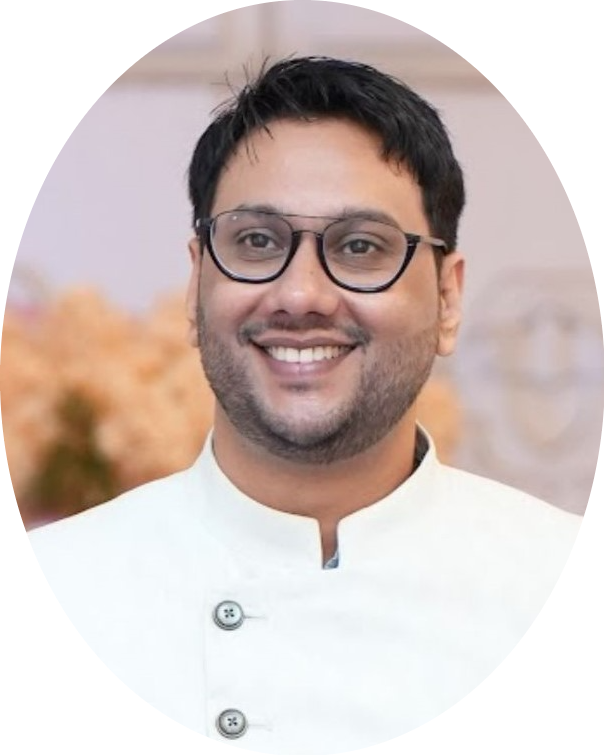
\includegraphics[width=\textwidth]{ResumePic-modified.png} % your image path
\end{minipage}
\par % End of the centering effect



%-------------------------------------------------------------------------------
% SUMMARY
%-------------------------------------------------------------------------------
\section*{{\textbf{\textcolor{blue}{SU}}\textbf{\textcolor{darktext}{MMARY}}}}
\hrule
Experienced Data Scientist with several years of track record in data science and analytics combined with software development, seeking the role of Data Scientist in AI domain. Proven experience in Python, R, and SQL. I bring hands-on experience in leveraging advanced statistical modeling, machine learning, deep learning and visualization 
 techniques for Stakeholder's vision.

%-------------------------------------------------------------------------------
% EXPERIENCE
%-------------------------------------------------------------------------------
\section*{{\textbf{\textcolor{blue}{EX}}\textbf{\textcolor{darktext}{PERIENCE}}}}
\hrule

\begin{itemize}[left=0pt]
  \item \textbf{Company 1} \hfill \textcolor{blue}{\emph{Remote, Germany}} \\
  \emph{Data Scientist \hfill from - till}
  \begin{itemize}
    \item Developed a predictive maintenance models using K-mean clustering and XgBoost for anomaly detection and electricity production and solar panel performance, achieving 18\% improvement in maintenance predictions and enhancement in real-time performance analysis.
    \item Deployed machine learning algorithms and Data pipelines using Airflow and AWS. 
    \item  Achieved a 0.8\% increase in model efficiency and a 3.5\% improvement in model accuracy.
  \end{itemize}
\end{itemize}

\begin{itemize}[left=0pt]
  \item \textbf{company 2} \hfill \textcolor{blue}{\emph{Palo Alto, CA, USA}} \\
  \emph{Senior Data Scientist \hfill from - till}
  \begin{itemize}
    \item Applied deep learning algorithms(Encoders, RNNs) using Python, developed state-of-the-art models for classification tasks on multi-modal datasets, and increased the precision and effectiveness of credit risk assessments by elevating model accuracy from 73\% to 81\%.
    \item Implemented Machine Learning and Deep Learning models in a production environment using Airflow, AWS and Github.
     
  \end{itemize}
\end{itemize}

\begin{itemize}[left=0pt]
  \item \textbf{Compnay 3} \hfill \textcolor{blue}{\emph{Sacramento, CA, USA}} \\
  \emph{Data Scientist \hfill from - till}
  \begin{itemize}
    \item Utilized sentiment analysis and data mining methods to examine customer responses, extracting valuable insights. 
    \item Used machine learning algorithms for predictive analysis to forecast time delays in load delivery, enhancing operational efficiency.
  \end{itemize}
\end{itemize}

\begin{itemize}[left=0pt]
  \item \textbf{Company 4} \hfill \textcolor{blue}{\emph{South Salem, NY,USA}} \\
  \emph{Data Scientist \hfill from - till}
  \begin{itemize}
    \item Developed a predictive model using RFM methodology for student dropout, leading to notable improvements in early identification of at-risk students and increased retention rates.
    \item Utilized sophisticated data processing and feature engineering techniques (ETL), incorporating factors such as attendance patterns, academic performance, and course engagement metrics to enhance
  \end{itemize}
\end{itemize}

\begin{itemize}[left=0pt]
  \item \textbf{Cpmpany 5} \hfill \textcolor{blue}{\emph{Noida, India}} \\
  \emph{Senior Business/Data Analyst \hfill from - till}
  \begin{itemize}
    \item Led data transformation initiatives, proficiently handling diverse formats of raw marketing data through various methods. 
    \item Crafted comprehensive model instructions and detailed reports for managers, encompassing variable explanations and scenario tests in predictive modeling.
  \end{itemize}
\end{itemize}

\begin{itemize}[left=0pt]
  \item \textbf{Company 6} \hfill \textcolor{blue}{\emph{Delhi, India}} \\
  \emph{Software Engineer \hfill from - till}
  \begin{itemize}
    \item Demonstrated expertise in SQL queries for meticulous data validation, aligning with Business Requirements Documents (BRDs).
  \end{itemize}
\end{itemize}

%-------------------------------------------------------------------------------
% EDUCATION
%-------------------------------------------------------------------------------
\section*{{\textbf{\textcolor{blue}{ED}}\textbf{\textcolor{darktext}{UCATION}}}}
\hrule
\begin{itemize}[left=0pt]
\item \textbf{State University of New York College} \hfill \textcolor{blue}{\emph{ City, Country}} \\
  \emph{M.Sc. in Data Science \hfill from - till}
\item \textbf{Technical University} \hfill \textcolor{blue}{\emph{Place, Country}} \\
  \emph{Bachelors of Science in Computer Science \hfill from - till}
\end{itemize}

%-------------------------------------------------------------------------------
% TECHNICAL SKILLS
%-------------------------------------------------------------------------------
\section*{{\textbf{\textcolor{blue}{TE}}\textbf{\textcolor{darktext}{CHNICAL SKILLS}}}}
\hrule
\begin{itemize}[left=0pt]
\item \textbf{AI/ML \& Deep Learning}: Advanced proficiency in Generative AI, Natural Language Processing, Regression, Decision Tree, Random Forrest, Supervised and Unsupervised learning, Large Language Models, Computer Vision and Forecasting, Hyper Parameter Tuning. %and Reinforcement learning.
\item \textbf{Cloud Services \& Solution Architecture}: Expertise in AWS AI services, AWS Datastores, AWS SageMaker,, Microsoft Azure, Docker,  Kubernetes, Airflow, Github. 
\item \textbf{Programming \& Software Engineering}: Python, R, SQL, HTML, CSS, Javascript, Typescript, REST API, Angular, scikit-learn, Pandas, Numpy, RNN, CNN, Transformers, Tensorflow, Keras.% Langchain, and OpenCV.
\end{itemize}

%-------------------------------------------------------------------------------
% FUNCTIONAL SKILLS
%-------------------------------------------------------------------------------
\section*{{\textbf{\textcolor{blue}{FU}}\textbf{\textcolor{darktext}{NCTIONAL SKILLS}}}}
\hrule
\begin{itemize}[left=0pt]
\item \textbf{Leadership}: Led cross-functional teams in various organizations, overseeing complex projects from start to finish.
\item \textbf{Communication}: Articulated complex AI/ML/DL concepts to both technical and non-technical stakeholders.
\item \textbf{Collaboration}: Effectively balanced the interests of both companies and customers in sensitive AI projects, ensuring mutually beneficial outcomes and enhanced stakeholder satisfaction. 
\item \textbf{Languages}: Proficient in English (Full Professional Proficiency) and German (A2 Level - Basic Proficiency)
\end{itemize}

%-------------------------------------------------------------------------------
% ACHIEVEMENTS
%-------------------------------------------------------------------------------
\section*{{\textbf{\textcolor{blue}{AC}}\textbf{\textcolor{darktext}{HIEVEMENTS}}}}
\hrule
\begin{itemize}[left=0pt]
\item Awarded for outstanding academic performance by State University of New York.
\item Co-authored two research papers/Poster for the Greater New York ACSM Spring Meeting 2019, focusing on healthcare analytics.
\end{itemize} 

\end{document}
